\chapter{Flow in Porous Media} \thispagestyle{chapterpage}
\label{chapter:flow_porous_media}
This chapter introduces petroleum reservoirs and the basic mathematical tools used to model fluid flow in porous media. We start out by giving a brief overview of porous media and petroleum reservoirs in Section \ref{section:introduction_petroleum_reservoirs}, before the mathematical model for fluid flow is developed from conservation principles and constitutive relations in Section \ref{section:reservoir_modeling}.

%%%%%%%%%%%%%%%%  INTRODUCTION TO PETROLEUM RESERVOIRS %%%%%%%%%%%%%%%%
\section{Introduction to Petroleum Reservoirs}
\label{section:introduction_petroleum_reservoirs}

\subsection{Porous media}
The term \emph{porous media} encompasses a wide range of physical media containing void space, quantified by the \emph{porosity} $\phi = \frac{\text{volume of void space in V}}{|V|}$, where $V$ is a connected region in the media at hand and $\vert V \vert$ is the volume of said region. Here the term \emph{void space} is interpreted as areas of the material matrix not occupied by the material itself, that is, areas where for example fluids can reside.  We also use the term \emph{pore space} for these volumes. The total available \emph{pore volume} in a rock sample is measured by the quantity $\vert V \vert\phi$, where $\phi$ is assumed to be a constant value for given regions of the media. Many seemingly solid everyday materials contain void space on a microscopic scale. Examples include wood, fabric, and, maybe more interesting, geological objects like rock and clay. Even ``solid'' rocks can contain a non-trivial void space, and it is in these cracks and crevices the hydrocarbon components in a petroleum reservoir are trapped. Void space in solid rock can be caused by either space between mineral grains, fractures, solution cavities in carbonate rock, or gas vesicles in volcanic rock \citep{jain_ch._2013}. Figure \ref{fig:pore_void_space} illustrates the void space for the mineral grain and fracture type pore volumes.

\begin{figure}[ht]
\begin{subfigure}[b]{0.49\textwidth}
	\centering
    	
\includegraphics[width=0.7\textwidth]{figures/mineral_grains.png}
	\caption{Mineral grains} \label{fig:pore_void_space_mineral_grains}
\end{subfigure}
\begin{subfigure}[b]{0.49\textwidth}
	\centering
	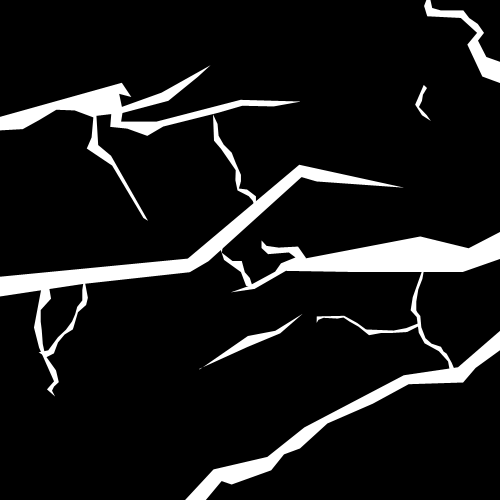
\includegraphics[width=0.7\textwidth]{figures/fractures.png}
	\caption{Fractures} \label{fig:pore_void_space_fractures}
\end{subfigure}
\caption{Illustration of volume between mineral grains and fracture voids in rocks. White color indicates void space where fluids can reside. Black color indicates mineral structures.}
\label{fig:pore_void_space}
\end{figure}

For so-called \emph{immiscible} (non-mixing) fluids the volume available for hydrocarbons, the \emph{hydrocarbon pore volume}, is limited by residual water in the pore space, called the \emph{irreducible water saturation} $S_{\text{wc}}$ of the rock \citep{dake_fundamentals_1978}. This water cannot be displaced by the hydrocarbon components, effectively reducing the available pore volume $\phi$ with a factor $S_{\text{wc}}$. Thus the hydrocarbon pore volume becomes $\vert V \vert \phi(1 - S_{wc})$. In the following it is assumed that the porosity is adjusted according to the irreducible water saturation, allowing us to use $\vert V \vert \phi$ for the hydrocarbon pore volume.

The porosity is obviously an essential parameter for a petroleum reservoir in that it limits the amount of space available for fluid components. What the porosity does not tell us about is the ease with which fluids flow through the formation. A rock with completely isolated pore spaces could in theory have a very high porosity, but without fluid flow between pore spaces oil and gas extraction would be impossible. Thus, the \emph{permeability} $\vec{K}$ of the rock is introduced \citep{jain_ch._2013}. $\vec{K}$ measures the degree of interconnectivity between the pore spaces. A high permeability indicates that it is easy for fluids to pass through the rock. As here, $\vec{K}$ is often given as a tensor since the media in which fluid flows can be anisotropic. That is, the permeability is directional dependent and varies between the different spatial directions. Table \ref{table:rock_permeabilities} shows a few typical absolute value permeability ranges, along with a classification and examples of rock types with the relevant properties. The table is modified from \citet{bear_dynamics_1972}.
\begin{table}
\caption{Typical permeability ranges for petroleum reservoir rock formations. Modified from source: Table 5.5.1 in \citep[p.~136]{bear_dynamics_1972}.} 
\label{table:rock_permeabilities}
\centering
\begin{tabular}{ M{2.5cm} | M{2.5cm} | M{4.5cm} N }
\bf{Permeability} 		      & \bf{Rocks} 			   & Range of $\log_{10}(K) [mD]$ &\\[1.1ex]\hline
Pervious 				      & Fracture rock 			   & $10^8$ to $10^4$   &\\[1.1ex]\hline
\multirow{2}{*}{Semipervious} & Oil Rock 	      			   & $10^4$ to $10$   &\\[1.1ex]\cline{2-3}
					      & \multirow{2}{*}{Sandstone}  & $10$ to $1$   &\\[1.1ex]\cline{1-1}\cline{3-3}
\multirow{3}{*}{Impervious}     & 					   & $1$ to $0.1$ &\\[1.1ex]\cline{2-3}
	 				      & Dolomite 				   & $0.1$ to $10^{-3}$ &\\[1.1ex]\cline{2-3}
 					      & Granite 				   & $10^{-3}$ to $10^{-5}$ &\\[1.1ex]\hline
\end{tabular}
\end{table}

The permeable regions where hydrocarbons flow are of little use if the valuable components escape to the surface. Laymen often think of oil and gas reservoirs as underground ``pools'' of fluids. The reality is not that far off, except that the geometry is inverses;  light petroleum components escape towards the surface and are trapped in an upside down pool by low-permeability geological formations, or in some cases by special hydrological phenomena \citep{jain_ch._2013}. Light components such as natural gas, if present, are found in the top layer, while the heavier oil is found just above the water aquifer in the bottom of the region.
%\begin{table}
%\centering
%\begin{tabular}{l | c | c | c | c | c | c}
%\bf{Permeability} & Pervious & \multicolumn{2}{ c | }{Semipervious} &  \multicolumn{3}{ c }{Impervious} \\
%\hline
%\bf{Rocks} & Fractured rock & Oil Rock &  \multicolumn{2}{ c | }{Sandstone} & Dolomite & Granite \\
%\hline
%$\log_{10}(K)$ [D] & [8,4] & [4,1] & [1,0] & [0,-1] & [-1,-3] & [-3,-5] \\
%\end{tabular}
%\caption{Typical permeability ranges for petroleum reservoir rock formations. Modified from source: Table 5.5.1 in \citep[p.~136]{bear_dynamics_1972}.} \label{table:rock_permeabilities}
%\end{table}
%%%%%%%%%%%%%%%% DRIVING MECHANISMS %%%%%%%%%%%%%%%%
\subsection{Driving Mechanisms of Production}
Petroleum components are harvested by drilling wells with perforations in the reservoir region, where pressure differences in the fluid drives it towards the surface. The natural pressure of the reservoir is often sufficient to drive the initial production. Continued production of hydrocarbon is driven by one or more of four mechanisms; solution gas drive, gas cap drive, natural water drive, and compaction drive \citep{dake_fundamentals_1978}. Removal of fluids from the reservoir causes a pressure drop. When the pressure is lowered compressible components expand and push the fluid components out of the rock formations. This is the cause of the three first drivers. In particular, gas drive is caused by expansion of oil and gas in solution. A lowering of pressure causes these components to precipitate and expand the volume of fluids, causing an evacuation of the rock formation. A gas cap or an aquifer, if present, will also expand under lowered pressure, again pushing down (or up in the case of water) on the oil strata and forcing it out of the reservoir region. The last driving mechanism, compaction drive, is caused by a collapse in the rock formation following the removal of supporting fluids. The collapse of the rock matrix forces remaining fluid out of the void space. All of these processes are part of the \emph{primary recovery} of the oil field. Primary recovery usually accounts for no more than $15\%$ of the oil in place \citep{tzimas_enhanced_2005}.

After the natural pressure drive of the reservoir weakens so called \emph{secondary recovery} is used. These techniques expend energy to increase the production potential of the reservoir. The most common secondary recovery technique is water injection, but other fluid types are also used. In the North Sea the primary and secondary oil recovery ranges between $45\%$ and $55 \%$ of original oil in place \citep{green_enhanced_2003}. 

The last category of the so called \emph{enhanced oil recovery} techniques, \emph{tertiary recovery}, seeks to alter the fluid and rock properties in the reservoir to improve the flow. These techniques are usually employed towards the end of the lifetime of a field, and are known to give an extra $5\%$ to $15\%$ of production \citep{tzimas_enhanced_2005}. It is worth noting that in modern petroleum reservoirs all three levels of recovery techniques are used in every part of the lifecycle of a field according to need, contrary to the hierarchical naming convention.

%%%%%%%%%%%%%%%% RESERVOIR MODELS %%%%%%%%%%%%%%%%
\section{Petroleum Reservoir Modeling}
\label{section:reservoir_modeling}
\begin{figure}
\centering
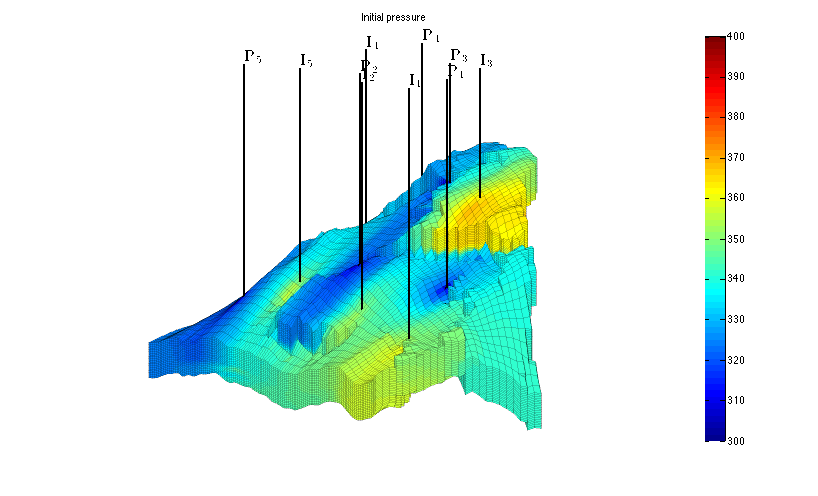
\includegraphics[trim=3cm 0cm 2cm 0cm,width=0.8\textwidth]{figures/saigup_field_pressure.png}
\caption{Example of a stratigraphic grid model of the Saigup field with wells and initial pressure data \citep{saigup_2003}.}
\label{fig:saigup_field_pressure}
\end{figure}
An oil reservoir is a complex and extensive structure. To run fluid simulations on the full scale model we need to identify and store the important properties of the rock formations together with information about the fluids contained within the hydrocarbon pore volume. These data points are gathered from the field by core samples, fluid samples, and seismic and electromagnetic geological exploration. The data gathered from field studies are compiled into a reservoir model containing all relevant parameters about the physical reservoir. Parameters like the permeability tensor $\vec{K}$, porosity $\phi$, phase saturation $S_l$ for phase $l$, and pressure $p$ are averaged and assigned to blocks representing subdomains of the model. This discrete version of the reservoir is closely connected to the discretized domain used when solving the fluid equations, as discussed in Section \ref{section:seq_splitting_method}. These static parameters represent the geological model, which (at least in our discussion) does not change throughout the lifetime of the field. The reservoir model also includes any injection or production wells and relevant well equations. An example of a grid on a rock formation is shown in Figure \ref{fig:saigup_field_pressure}. Here, the wells are shown as black lines and the pressure in each cell is indicated with color. This example uses a typical \emph{stratigraphic} grid, which allows for a semi-structured grid while retaining the layered nature of the rock formations. It is on such discrete versions of the domain we will develop the flow equations. The reservoir model also includes a \emph{fluid model}, a set of principles and equations chosen to model the hydrocarbon and water components present in the rock formations. Finally, the external interfaces of the reservoir are described. These include production and injection wells, and any fluxes across the outer boundaries of the reservoir, although \emph{no-flow boundaries} are usually assumed. We start by deriving a \emph{continuity equation} from the principle of \emph{mass conservation}.

%%%%%%%%%%%%%%%% THE CONTINUITY EQUATION %%%%%%%%%%%%%%%%
\subsection{The Continuity Equation}
\label{section:continuity_equation}
Conservation of mass is an important concept in fluid dynamics. It effectively states that mass can be neither created nor destroyed. This implies that the amount of mass in a closed system is constant. Here "closed" is taken to mean closed to mass and energy transfer, since thermodynamical processes also cause mass transfer according to the principle of \emph{mass-energy equivalence}.
%\citep{einstein_considerations_1940}
Even for thermodynamically open systems the conservation of mass is a relatively good approximation at reasonable energy levels. The continuity equation follows from conservation of mass by considering a \emph{control volume} $V \subset \mathbb{R}^d$, $d \in \{1,2,3\}$, over which we track mass exchange, see Figure \ref{fig:control_volume} for an example in two dimensions ($d = 2$). For a material with density $\rho$ we can compute the mass $m$ in the control volume at time $t$ by a volume integral of $\rho(\vec{x},t)$ over $V$, where $\vec{x} \in \mathbb{R}^d$ is a point in $V$:
\begin{equation*}
m = \int \limits_{V} \rho(\vec{x},t) \differential{V}.
\end{equation*}
If the concentration of some quantity in $V$ is measured by $\varphi$ we can do a similar integral and compute the amount in the control volume at time $t$ by
\begin{equation*}
\varphi_V(t) = \int \limits_{V} \varphi(\vec{x},t)\rho(\vec{x},t) \differential{V}.
\end{equation*}
This assumes that the conserved quantity is chemically inert, i.e., that there is no mass transfer between the conserved material and the other components in the control volume, and that no sources are present.
\tikzsetnextfilename{control_volume_V}
\begin{figure}[ht]
\centering
\begin{tikzpicture}
    \node[anchor=south west,inner sep=0] (image) at (0,0) {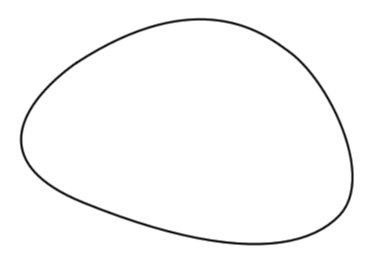
\includegraphics[width=0.5\textwidth]{figures/controlVolume.png}};
    \begin{scope}[x={(image.south east)},y={(image.north west)}]
        \node [left] at (0.5,0.5) {$V$};
        \node [right] at (0.85,0.79)  (normal) {$\vec{\nu}$};
        \draw [ultra thick, ->] (0.84,0.70) -- (0.95,0.80);
        \node [right] at (0.92,0.59) (flux) {$\vec{f}$};
        \draw [ultra thick, ->] (0.84,0.70) -- (1.07,0.65);
    \end{scope}
\end{tikzpicture}
\caption{A control volume $V \subset \mathbb{R}^2$ with boundary $\partial V$, unit surface normal $\vec{\nu}$ and a flux $\vec{f}$.}
\label{fig:control_volume}
\end{figure}
We now open the boundary $\partial V$ of $V$ and start tracking the mass transfer out of the control volume. The movement across $\partial V$ sets up a flux $\vec{f}$. Letting $\differential{\vec{v}}$ be an infinitesimal part of $\partial V$ with an outward facing unit normal $\vec{\nu}$ we can compute the mass transfer by
\begin{equation*}
 \int \limits_{\partial V} \vec{f} \cdot \vec{\nu} \differential{\vec{v}},
\end{equation*}
where $\vec{f} \cdot \vec{\nu}$ is the transport of the preserved quantity across $\differential{\vec{v}}$. Further, the change in the concentration of the preserved quantity within $V$ is measured by the temporal derivative of $\varphi_V(t)$:
\begin{equation*}
\frac{\partial \varphi_V(t)}{\partial t} = \text{change in $\varphi_V(t)$ during $\differential{t}$}.
\end{equation*}
Sources, either negative (sinks) or positive (sources), are introduced through a source term $q(\vec{x},t)$. Integrating over the control volume gives the total source term $q_{\text{tot}} = \int_V q(\vec{x},t) \differential{V}$. By convention, $q > 0$ is treated as an injection into the control volume. We now arrive at the complete conservation principle as applied to the control volume $V$:
\begin{equation} \label{eq:conservation_principle}
\frac{\partial \varphi_V(t)}{\partial t} = \int\limits_{V} q(x,t) \differential{V} - \int \limits_{\partial V} \vec{f} \cdot \vec{\nu} \differential{v}.
\end{equation}
We now use the \emph{divergence theorem}, see e.g. \citep[p.~68-69]{weber_essential_2003}, to relate the boundary flux to the divergence inside the control volume:
 \begin{equation} \label{eq:divergence_theorem}
 \int \limits_{\partial V} \vec{f} \cdot \vec{\nu} \differential{v} = \int \limits_{V} \nabla \cdot \vec{f} \differential{V}.
 \end{equation}
The boundary flux term now transforms directly to a control volume formulation, allowing us to gather the terms in the same integral, giving
\begin{equation*}
 \int \limits_{V} \left[ \frac{\partial{}}{\partial{t}} \left[ \varphi(x,t)\rho(x,t) \right] + \nabla \cdot \vec{f} - q(x,t) \right] \differential{V} = 0.
\end{equation*}
This works under the assumption of sufficient smoothness of the flux (for the divergence theorem) and the concentration and density (for the time derivative to move inside the integral), and by the linearity of the integral operation. Finally we arrive at the \emph{continuity equation} for the quantity of concentration $\varphi$:
\begin{equation} \label{eq:general_conservation_equation}
\frac{\partial{}}{\partial{t}} \left[ \varphi(x,t)\rho(x,t) \right] + \nabla \cdot \vec{f} = q(x,t).
\end{equation}
Here we have used the fact that the control volume $V$ is chosen arbitrarily, which implies that we can drop the integral sign without destroying the equality. If needed the source term can be modified to track mass transfer between components. The mass conservation relation results from Equation (\ref{eq:general_conservation_equation}) by setting $\varphi = 1$ and defining the mass flux $\vec{f} = \rho \vec{u}$, where $\vec{u}$ is the fluid velocity. Using a subscript for the time derivative we get the mass continuity equation:
\begin{equation} \label{eq:mass_conservation_equation}
\rho_t + \nabla \cdot \left( \rho \vec{u} \right) = q.
\end{equation}

So far we have assumed that the fluid phases can fill the control volume $V$ completely. As mentioned before, the porosity $\phi$ of the rock formations in the reservoir measures the available pore space. The porosity can be introduced into the continuity equation by letting it scale the total mass in the control volume, giving 
\begin{equation} \label{eq:mass_conservation_equation_porosity}
\left( \phi \rho \right)_t + \nabla \cdot \vec{f} = q.
\end{equation}
Here the temporal and spatial arguments are dropped for brevity. Equation (\ref{eq:mass_conservation_equation_porosity}) only models a single fluid \emph{phase}. A more advanced fluid description is introduced in the next section. 

%%%%%%%%%%%%%%%%  FLUID MODELS %%%%%%%%%%%%%%%%
\subsection{Fluid Models}
\label{section:fluid_models}
An important part of the reservoir model is the fluid description. The crude oil usually contains dissolved gas and the presence of a water phase is also common. A standard approach to fluid modeling is to use a compositional model where each hydrocarbon component, or at least a pseudo-component combining several chemical species, is subject to a mass balance equation. The fluid is described using three phases; the water, liquid and gas phase. In addition we introduce the mass fractions $C_{kg}$ and $C_{ko}$, that is, the mass fraction of component $k$ present in the gas and oil phase, respectively. Now the conditions $\sum_{k=1}^{n_c} C_{k \alpha} = 1, \alpha = \{g,o\},$ hold for a system with $n_c$ components. The mass-balance equations become
\begin{equation*}
( \phi (C_{kg} \rho_g S_g + C_{ko} \rho_o S_o) )_t + \nabla \cdot (C_{kg} \vec{f}_g + C_{ko} \vec{f}_o) = q_k,
\end{equation*}
for all components $k$, in addition to a standard continuity equation for water. The compositional fluid model will not be pursued further here.

At surface pressure and temperature the fluids from the reservoir separate into three phases; oil, gas, and water. The \emph{black-oil model} assumes that this holds in the reservoir too. Three pseudo-phases are assumed; a liquid phase, a gaseous phase, and a water phase. The black-oil model includes gas in solution through the \emph{solution gas-oil ratio}:
\begin{equation*}
R_{so} = \frac{\text{volume of gas evolved from oil at std. conditions}}{\text{volume of oil at std. conditions}}. 
\end{equation*}

$R_{so}$ is used to modify the density of the oil phase in order to account for the dissolved gas. Assuming three fluid phases implies three conservation laws, one for each phase. We model each of these phases by defining the \emph{phase saturation} $S_l$ of phase $l \in \{w,g,o\}$, denoting water, gas, and oil, respectively. The saturation of a phase measures the ratio of the amount of fluid of the given phase to the available hydrocarbon pore volume in the control volume $V$. The restriction 
\begin{equation} \label{eq:saturation_constraint}
\sum_l S_l = 1,
\end{equation} 
called the \emph{saturation constraint}, is rather obvious since we assume that the phases fill the entire available pore volume. In the two phase case the restriction becomes $S_w + S_o = 1$. Introducing the phase saturation into Equation (\ref{eq:mass_conservation_equation_porosity}) produces the phase continuity equation
\begin{equation} \label{eq:continuity_phase}
( \phi S_l \rho_l )_t + \nabla \cdot \vec{f}_l = q_l.
\end{equation}
Since the oil can contain gas in solution we need to modify the densities accordingly. Introducing the oil and gas density at standard condition, $\rho_{o}^{s}$ and $\rho_{g}^{s}$, respectively, the liquid oil density $\rho_{o}^{l}$ and the gaseous oil density $\rho_{o}^{g}$, we can express the reservoir density of oil as 
\begin{equation*}
\rho_o = \frac{\rho_o^s+\rho_g^s R_\text{so}}{B_o} = \rho_{o}^{l} + \rho_{o}^{g}, 
\end{equation*}
where $B_o$ is the \emph{formation volume factor}, the ratio of volume of oil at reservoir conditions to the volume of oil at standard (surface) conditions. That is,
\begin{equation*}
B_{o} = \frac{\text{volume of oil at reservoir conditions}}{\text{volume of oil at std. conditions}}. 
\end{equation*}
This gives the following set of black oil equations which we will use, where gas in solution is taken into account:
\begin{subequations}
\label{eq:black_oil_model}
\begin{align}
( \phi S_w \rho_w )_t + \nabla \cdot \vec{f}_w &= q_w, \\
( \phi S_o \rho_{o}^{l} )_t + \nabla \cdot \vec{f}_o &= q_o, \\
( \phi S_g \rho_g + \phi S_o \rho_{o}^{g} )_t + \nabla \cdot \vec{f}_l &= q_g.
\end{align}
\end{subequations}
